\chapter{Physical Object Reconstruction}\label{ch:reco}

Physical properties of particles produced from a collision at the \ac{lhc} are derived by combining the traces these particles leave in the various subdetectors as they traverse \ac{atlas}. The upcoming sections will describe the reconstruction processes for various objects utilized in this analysis. The primary reference for this chapter is \citep{atlas2021optimisation}.

\section{Tracks and Primary Vertex}\label{sec:tracks}
Charged particles leave a trajectory in the \ac{id} as explained in the section \ref{sec:inner_detector}. To reconstruct the path of these particles an algorithm first groups hits that are close to each other in the silicon detectors into clusters. These clusters are then successively combined to determine the most probable trajectory that the particles have taken through the detector which are referred to as tracks \citep{aaboud2017performance}. These are then geometrically matched to proton-proton interactions and the vertex with the largest scalar sum of transverse momenta $\sum \pt^2$ is identified as the primary hard scatter vertex. In addition, the momentum is also determined based on the curvature of the particle through the magnetic field and at least two tracks with $\pt>\qty[]{500}{MeV}$ are required to be in the tracking volume $\abs{\eta}<2.5$.

\section{Jets}\label{sec:jets}
As discussed in section \ref{sec:renormalization} quarks cannot be observed individually but only as colorless hadrons. When decaying they undergo showering and hadronization forming cone-like structures of energy deposits in the detector called jets. They are reconstructed by combining and grouping tracking and calorimeter information.

\subsection{Topocluster}
The deposited energy of decays in the calorimeters are grouped three-dimensionally by combining calorimeter cells into so-called topoclusters. These clusters are seeded from cells that display a signal stronger than four times the standard deviation of detector noise $4\sigma_\mathrm{noise}$ encompassed by $2\sigma_\mathrm{noise}$ cells.

\subsection{Particle Flow Object}\label{sec:particle_flow}
The energy and mass resolution calculated from topoclusters can be improved by geometrically matching tracks to the clusters. This exploits the momentum and position resolution of the \ac{id} to complement the energy measurements obtained from the calorimeter. When a track is successfully matched to a topocluster, the expected energy, based on the particle that created the track, is computed. From this expected energy all associated cluster cell energies are subtracted and the remnant is removed from the expected energy if energy is within the range of typical fluctuations. Such combination of a topocluster and a track are called \ac{pfo} \citep{aaboud2017jet}. Sometimes energy of one track ends up in several clusters. For this the Particle Flow algorithm combines the most probable clusters with the track. Topoclusters without matched tracks are assumed to be neutral particles as they do not leave a trace in the \ac{id}. \acp{pfo} not matched to the \ac{pv} are removed to reduce the contribution from pileup.  This technique, especially in the reconstruction of low \pt clusters, enhances the overall resolution.

\subsection{Track-CaloClusters}
Instead of using the energy measurement of the tracks as for \acp{pfo} for \ac{tcc} the calorimeter energy measurement is used and complemented by the angular information of the tracks. \ac{tcc} was developed for high \pt jets since the resolution in the calorimeters improves with larger momentum since the calorimeter deposits become more localized.

% \subsection{Unified Flow Object}
% Particle Flow benefits from the momentum/energy resolution of the \ac{id} compared to the calorimeters especially at low momenta. Although this gradually breaks down with increasing momentum and also with particle density because the matching of tracks to clusters becomes more and more ambiguous in that case. \ac{ufo} jets are designed to make the most of both reconstruction algorithms by choosing the algorithm that performs best for the situation at hand.

\subsection{Anti-$k_t$ Jet Clustering Algorithm}\label{sec:anti_kt}
The definition of a jet is not unique as it depends on the size and direction of the cone and thus how many particles are included. For this the Anti-$k_t$ algorithm \citep{cacciari2008anti} clusters aforementioned four vector objects in this section into cone-shaped jets. It starts with calculating the distances between all four vector objects $i,j$ that are considered
\begin{equation}
  d_{ij}=\frac{1}{\max(p_{T,i}^{2}\,,\,p_{T,j}^{2})} \frac{\Delta R_{ij}^2}{R^2},
\end{equation}
and the distance to the beam
\begin{equation}
  d_{iB}=\frac{1}{p_{T,i}^{2}},
\end{equation}
with the transverse momenta of the particles $p_{T,i},p_{T,j}$ their angular distance $\Delta R$ as of equation \ref{eq:delta_R} and a chosen radius parameter $R$. The algorithm combines objects $i,j$ into a new four vector for the smallest distance $d_{ij}$. The distance is small for large transverse momenta \pt and small angular distances $\Delta R_{ij}$ and are therefore preferred by the algorithm. After combining two objects the algorithm starts for as long as $d_{iB}<d_{ij}$. Thus it stops once particles outside of the chosen radius would be added. In \ac{atlas} jets with a radius parameter of $R=0.4 (1.0)$ are usually denoted as Small-R(Large-R) jets.


\subsection{Variable Radius Jets}\label{sec:vr_jets}
In very boosted regimes mit large momenta individual jets can overlap. In order to still reconstruct them individually a \ac{vr} for the $R$ parameter from the Anti-$k_t$ Jet Clustering Algorithm of section \ref{sec:anti_kt} is used
\begin{equation}
  R\rightarrow R_\text{eff}(\pt)=\frac{\rho}{\pt}
\end{equation}
It becomes therefore dependent on the transverse momentum and is controlled by a parameter $\rho$ so that the jet size decreases with \pt. \ac{vr} jets are reconstructed from tracks and are required to have $\pt>\qty[]{10}{GeV}$.

\section{$b$-tagging}\label{sec:b_tagging}
This analysis has four $b$-quarks in the final state and therefore relies on their identification.One of the key characteristics of $b$ quarks is their relatively large mass resulting in a long lifetime compared to other quarks $\tau\sim\qty{1.5}{ps}$. This translates to a decay length of about $c\tau \sim \qty{450}{\micro m}$ and leads to a secondary vertex. Although these $b$-hadrons do not reach the \ac{id} directly their decay positions can be deduced from tracks.

Such tracks have a large impact parameter that is defined as the distance of closest approach in the $r-\phi$ projection in transverse $d_0$ and longitudinal $z_o$ direction \citep{aad2008atlas} as illustrated in figure \ref{fig:secondary_vertex}b. Other methods for determining the secondary vertex attempt to connect the tracks of the $b$-hadron decay with those of a subsequent $c$-hadron decay by aligning the tracks in Fig. \ref{fig:secondary_vertex}a and also by deriving the mutual origins of the tracks \citep{ATL-PHYS-PUB-2017-013}.
\begin{figure}[]
  \centering
  \subfigure[]{
    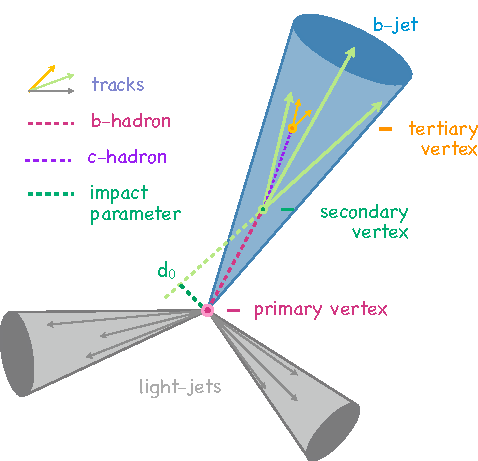
\includegraphics[width=0.49\textwidth]{secVexMguth}
  }%\hspace*{1cm}
  \subfigure[]{
    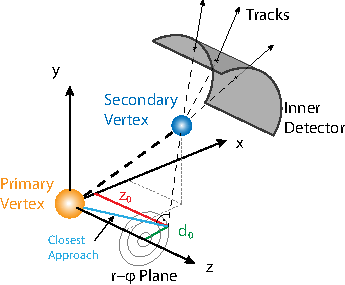
\includegraphics[width=0.49\textwidth]{SV_sketch}
  }
  \caption{(a) Example decay involving a $b$-jet (\hexbox{8AB2D3}) and jets from light flavor hadrons (\hexbox{C5C6C6}). (b) Impact parameters defined for tracks as distance of closest approach to the primary vertex for (\mbox{\color[HTML]{009245}{$d_0$}}) in the $r-\phi$-plane and for (\mbox{\color[HTML]{EC1C25}{$z_0$}}) along the z axis. (a) Adopted from \cite{Guth:2765038}.}
  \label{fig:secondary_vertex}
\end{figure}

\subsection{DL1d Tagger}
The results of the secondary vertex- and impact parameter finding algorithm as well as the jet kinematics are then passed into a deep feed-forward neural network called DL1d which is trained to distinguish $b$-jets from jets of other flavors \citep{atlas2022atlas}. The output nodes for flavor classification ($p_\mathrm{b}, p_\mathrm{c}, p_\mathrm{light}$) are further combined into a single discriminating score variable
\begin{equation}
  D_\mathrm{DL1d}=\ln\left(\frac{p_b}{f_c \cdot p_c + (1-f_c)\cdot p_\mathrm{light} }\right).
\end{equation}
$f_c$ is the fraction of charm jets in the background and can be used to tune the importance of the different background classes ($\sum f_\mathrm{bkg} =1$). When evaluating the \ac{nn} a value for the discriminating variable $D$ can be derived that corresponds to a $b$-jet selection efficiency which is then applied in physics analysis.

\subsection{$X\rightarrow bb$ Tagger}\label{sec:xbb}
For a collision event with decay products consisting of $b$-jets with large transverse momenta, jets reconstructed with a fixed radius parameter can become overlapped. To address such scenarios, \ac{vr} track jets, as discussed in Section \ref{sec:vr_jets}, can be reconstructed within a large-$R$ jet that encompasses both $b$-jets. The \ac{vr} jets are required to have $\rho=\qty[]{30}{GeV}$ a radius parameter constrained to $0.02 <R<0.4$. Further the \ac{vr} jets are not allowed to overlap. These parameters are optimized for Higgs to $bb$ decays \citep{ATL-PHYS-PUB-2017-010}.

The $X\rightarrow bb$ tagger is a feed-forward \ac{nn} \citep{ATL-PHYS-PUB-2020-019}. The inputs include the transverse momentum \pt and pseudorapidity $\eta$ of the large-$R$ jet along with outputs from DL1d for up to three \ac{vr} track jets. Similar to DL1d, a discriminant is computed from the \ac{nn}'s output scores, which reflect the likelihood of the event being a Higgs, top, or multijet decay:
\begin{equation}
  D_{\text{Xbb}}=\ln\left({\frac{p_{\text{Higgs}}}{f_{\text{top}}\cdot p_{\text{top}}+(1-f_{\text{top}})\cdot p_{\text{multijet}}}}\right).
\end{equation}
$f_\text{top}$ denotes the top fraction with regards to the multijet output. From the evaluation of the discriminant \acp{wp} are defined depending on the Higgs tagging efficiency.

\section{Jet Calibration}\label{sec:calibration}
Every measuring instrument must be calibrated In the case of jet reconstruction the main causes of discrepancies between the properties of jets inferred from reconstruction and their true properties include \citep{atlas2011jet}:
\begin{itemize}
  \item Non-Compensation: smaller calorimeter response of non-\ac{em} to particles of hadron showers than to \ac{em}
  \item Dead material: energy is deposited in non-instrumented areas
  \item Particles belonging to a decay but are outside of the reconstruction cone.
  \item Energy deposition below the noise threshold
  \item Particles from pile-up
  \item Leakage: particles are not stopped inside the calorimeter (punch-through)
\end{itemize}
To mitigate these effects there are several algorithms employed that also account for the detector geometry and are described in the following based on \citep{atlas2021jet}. As reference objects serve well-understood physics processes that leave a distinct signature in the detector like dijet events or decays of $Z$-bosons or photons.

\subsection{Pilup mitigation}
When bunches of protons are collided, not only one but rather several proton-proton interactions are measured. Various methods have been developed to separate these numerous interactions and are described for both small and large $R$ jets. Pile-up is categorized into in-time pile-up referring to additional proton-proton collisions occurring within the same bunch-crossing and out-of-time pile-up collisions occurring before and after the collision of interest. Over time these methods have seen significant improvements allowing for an increase in the mean number of interactions commonly referred to as pile-up. This increase in pile-up during the data taking period is depicted in Figure \ref{fig:pileup}.
\begin{figure}
  \centering
  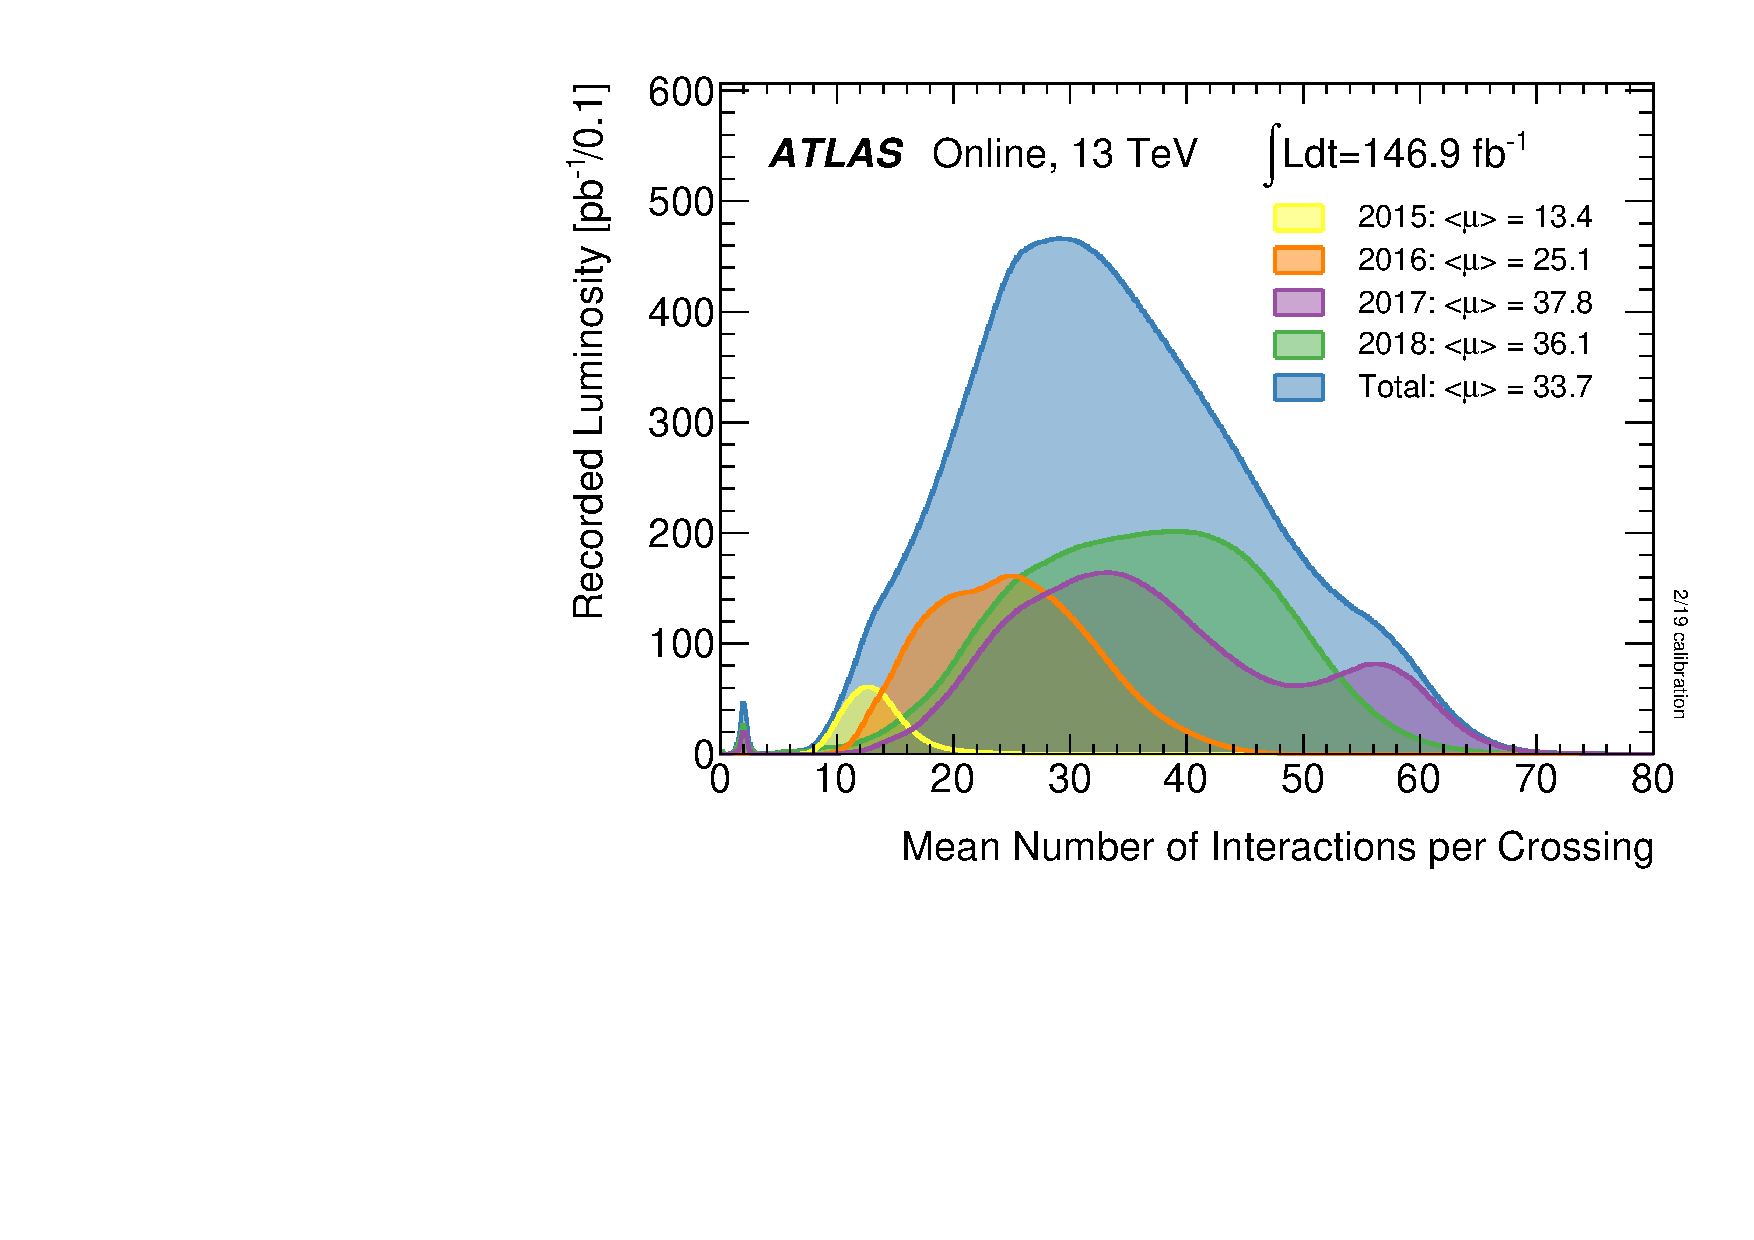
\includegraphics[width=0.5\textwidth]{mu_2015_2018}
  \caption[]{Pile up profiles for run 2 data taking periods \citep{pileup}.}
  \label{fig:pileup}
\end{figure}


\subsubsection{Small-R Jets}
At a first step contributions from pileup are reduced by subtracting the median transverse momentum density $\rho=\pt / A$ of jets found within $\eta<2.0$ multiplied by the active area of the jet $A_T$ as defined in \textsc{FastJet} \citep{cacciari2012fastjet}. Another reduction observes that the pileup corrected \pt is a function of the number of primary Vertices $N_\text{PV}$ and the mean number of interactions $\mu$. Thus the corrected transverse momentum is expressed as 
\begin{equation}
  \pt^\text{corr}=\pt-\rho A_T -\alpha(N_\text{PV}-1)-\beta\mu
\end{equation}
with parameters $\alpha$ and $\beta$. The effect of the correction is shown in figure \ref{fig:jet_pt_correction}.
\begin{figure}
  \centering
  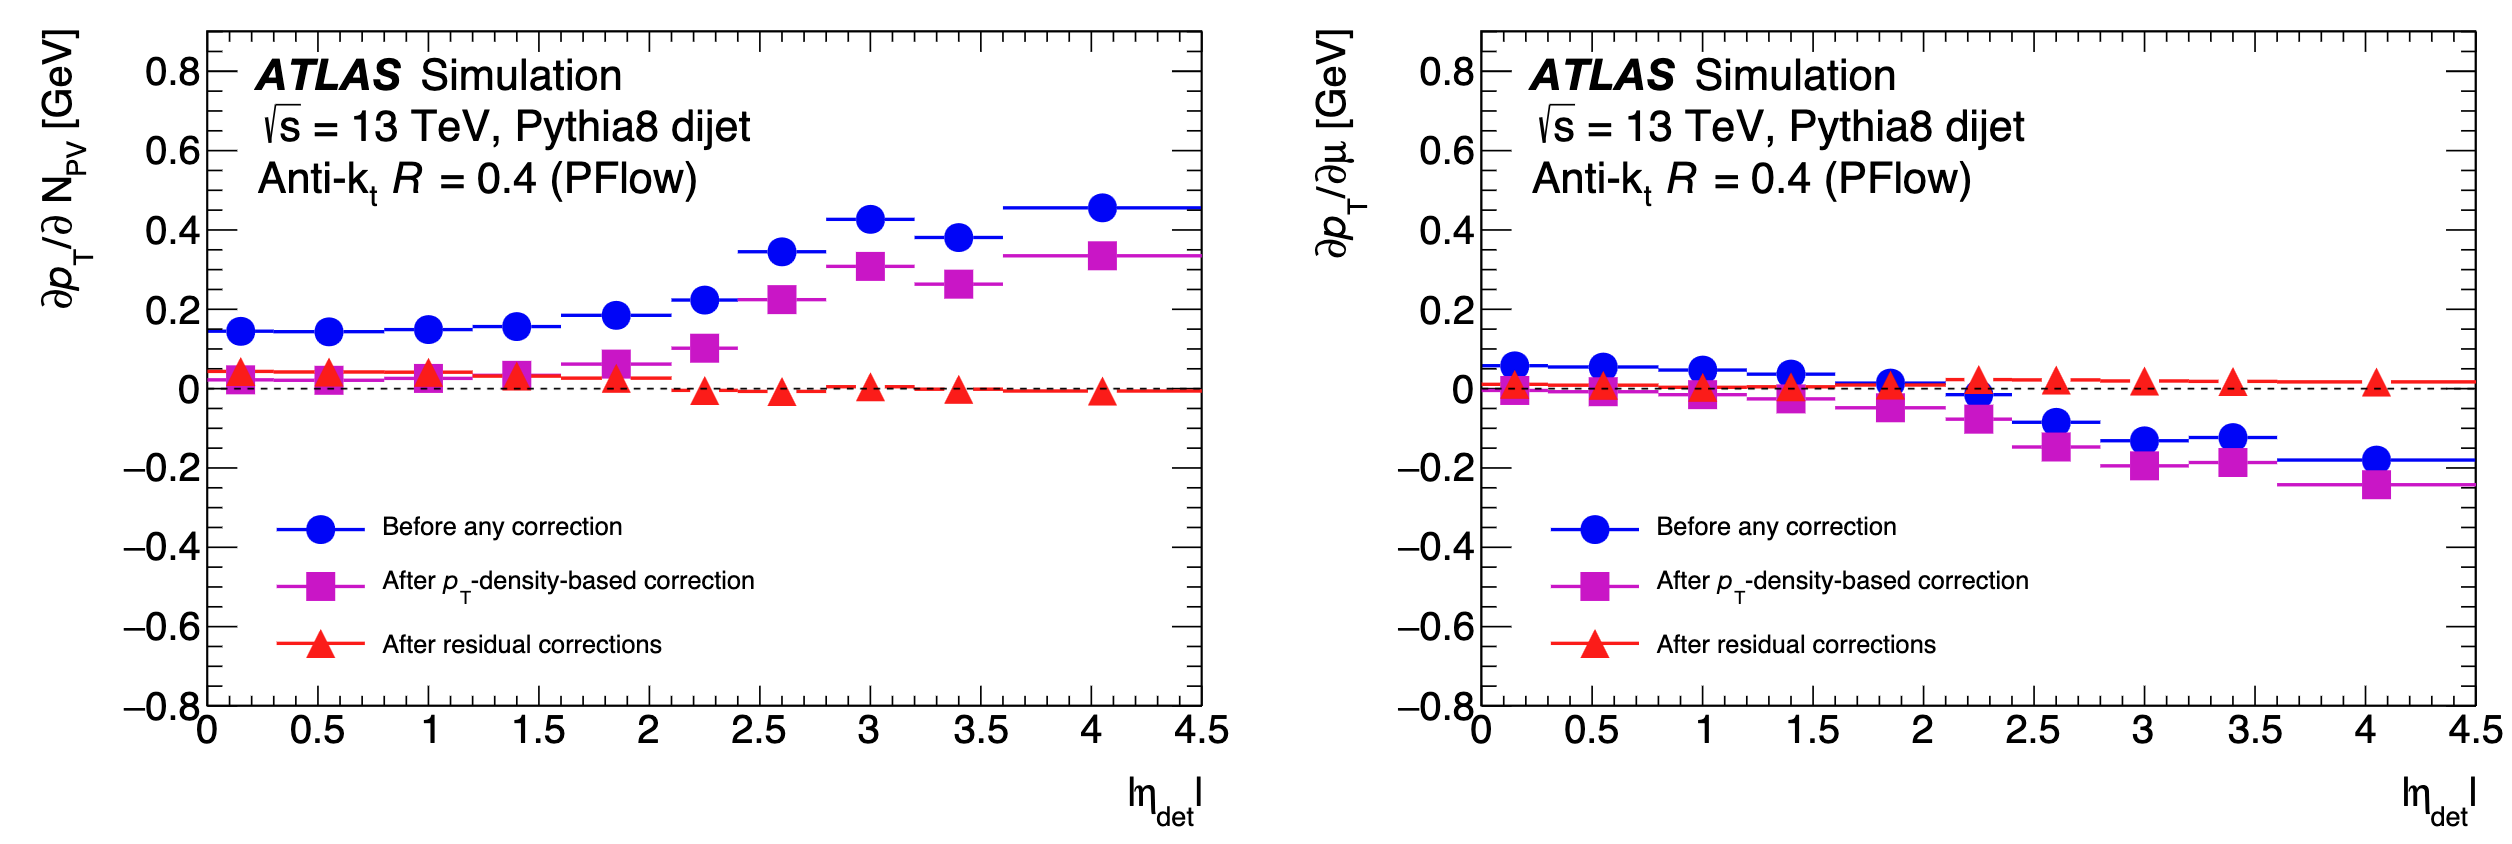
\includegraphics[width=1\textwidth]{jet_pt_correction}
  \caption[]{\pt correction to remove the \pt dependence of the jet at different $\eta$ for the \pt dependent on (left) the number of primary vertices and (right) average number of interactions of the collision.}
  \label{fig:jet_pt_correction}
\end{figure}

Moreover pileup contributions can be further reduced by comparing the scalar \pt sum of tracks from the \ac{pv} associated to the jet with the scalar \pt sum of all tracks including other \acp{pv}. The \ac{jvt} \citep{ATLAS-CONF-2014-018} utilizes this property to apply a quality criterion on jets with $\pt<\qty[]{60}{GeV}$ and $|\eta|<2.4$.


\subsubsection{Large-R Jets}
Due to their large surface area, large-$R$-jets are particularly susceptible to pile-up contributions. To counteract this, a technique known as grooming is used. In this process, a large $R$-jet is divided into smaller sub-jets with a radius of $R=0.2$. Of these subjets, only those that contain at least $\pt>\qty[]{5}{\percent}$ of the original large-$R$ jet are retained.

\subsection{\ac{jes}, $\eta$ and mass}
\begin{figure}
  \centering
  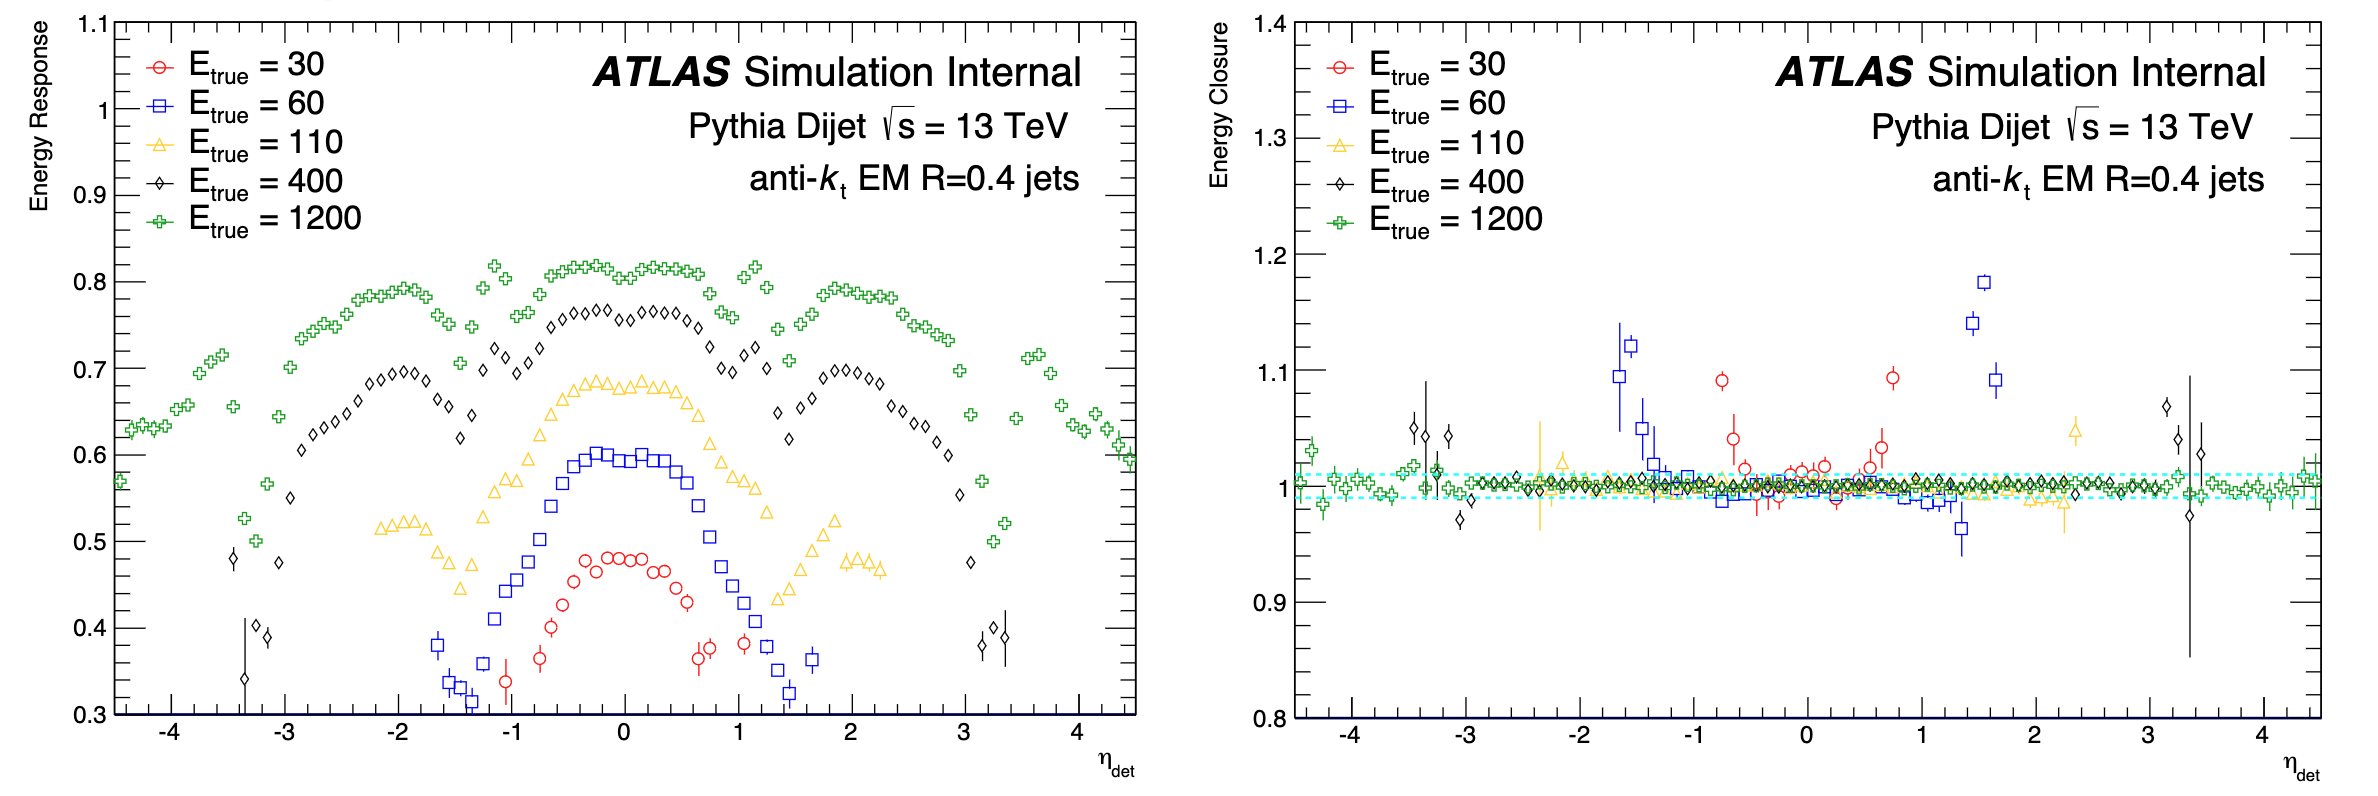
\includegraphics[width=1\textwidth]{jet_eta_mismatch}
  \caption[]{Jet energy response $E_\text{reco}/E_\text{truth}$ for different detector $\eta$ values (left) before and after applying (right) the calibration. Adopted from \citep{jet_eta_calib}.}
  \label{fig:jet_eta_mismatch}
\end{figure}
A clear mismatch between reconstructed and truth energy of simulated two jet events can be seen in the left plot of figure \ref{fig:jet_eta_mismatch} measured in $\eta$ bins. Based on this a continuous correction function in $\eta$ is derived and applied to correct for differences in jet energy, $\eta$ and mass \citep{atlas2011jet,Aaboud:2019aa}. This is exemplified in the right hand plot of figure \ref{fig:jet_eta_mismatch}.

\subsection{Global Sequential Calibration}
This step corrects the jet \pt without changing the mean energy of the jet. It corrects for non-compensation, dead material and leakage effects by using observables like the charged particle fraction, energy fractions in different calorimeter layers, track-related quantities and the muon activity behind the calorimeter. Corrections are again derived in \pt and $\eta$ and are applied sequentially.

\subsection{In situ calibration}
At the final step differences between data and simulation are corrected for in \pt. These variations stem from imperfect simulations of detector materials and the modeling of the involved physics processes. For this well known physics processes are used and correction factors are extracted in \pt. This step is only applied to data.

\subsection{Jet Event Cleaning}
Another method to reduce background is called event cleaning. It removes the whole event if jets are found that where generated by out-of-time pileup, cosmic rays or beam-induced backgrounds by applying a set of quality criteria to variables describing the jet profile \citep{ATLAS-CONF-2015-029}.

\subsection{Mass correction for Large-$R$ jets}
The mass of a jet is calculated from the energy deposits in calorimeter clusters $i$ via
\begin{equation}
  m_{\text{calo}} = \sqrt{\left(\sum_{i\in \text{Jet}}E_i\right)^2-\left(\sum_{i\in \text{Jet}}\vec{p_i}\right)^2}.
\end{equation}
For very boosted jets the spread of particles inside the jet can become the size of the granularity of the calorimeter and the energy resolution degrades accordingly. With the help of tracking information from the \ac{id} the energy and mass resolution can be improved across the whole \pt range \citep{Aaboud:2019aa}. The track assisted jet mass is then
\begin{equation}
  m_{\text{TA}} = \frac{p_{\text{T}}^{\text{calo}}}{p_{\text{T}}^{\text{track}}} \cdot m_{\text{track}}
\end{equation}
where $p_{\text{T}}^{\text{calo}}$ is the transverse momentum measured in the calorimeter, $p_{\text{T}}^{\text{track}}$ is the transverse momentum of the four-vector sum of tracks associated to the large-$R$ jet and $m_\text{track}$ is the invariant mass of this four-vector sum of tracks. Since the \ac{id} is only susceptible to charged particles the ratio of $p_{\text{T}}^{\text{calo}}$ and $p_{\text{T}}^{\text{track}}$ scales the mass measured from tracks to include neutral particles. The improvement is visualized in figure \ref{fig:combined_mass_large_R}. The calorimeter and track-assisted mass measurement are then linearly combined with a weight $w$ to give optimal results
\begin{equation}
  m_{\text{comb}} =  w\cdot m_{\text{calo}}+(1-w)\cdot m_{\text{TA}}.
\end{equation}
\begin{figure}
  \centering
  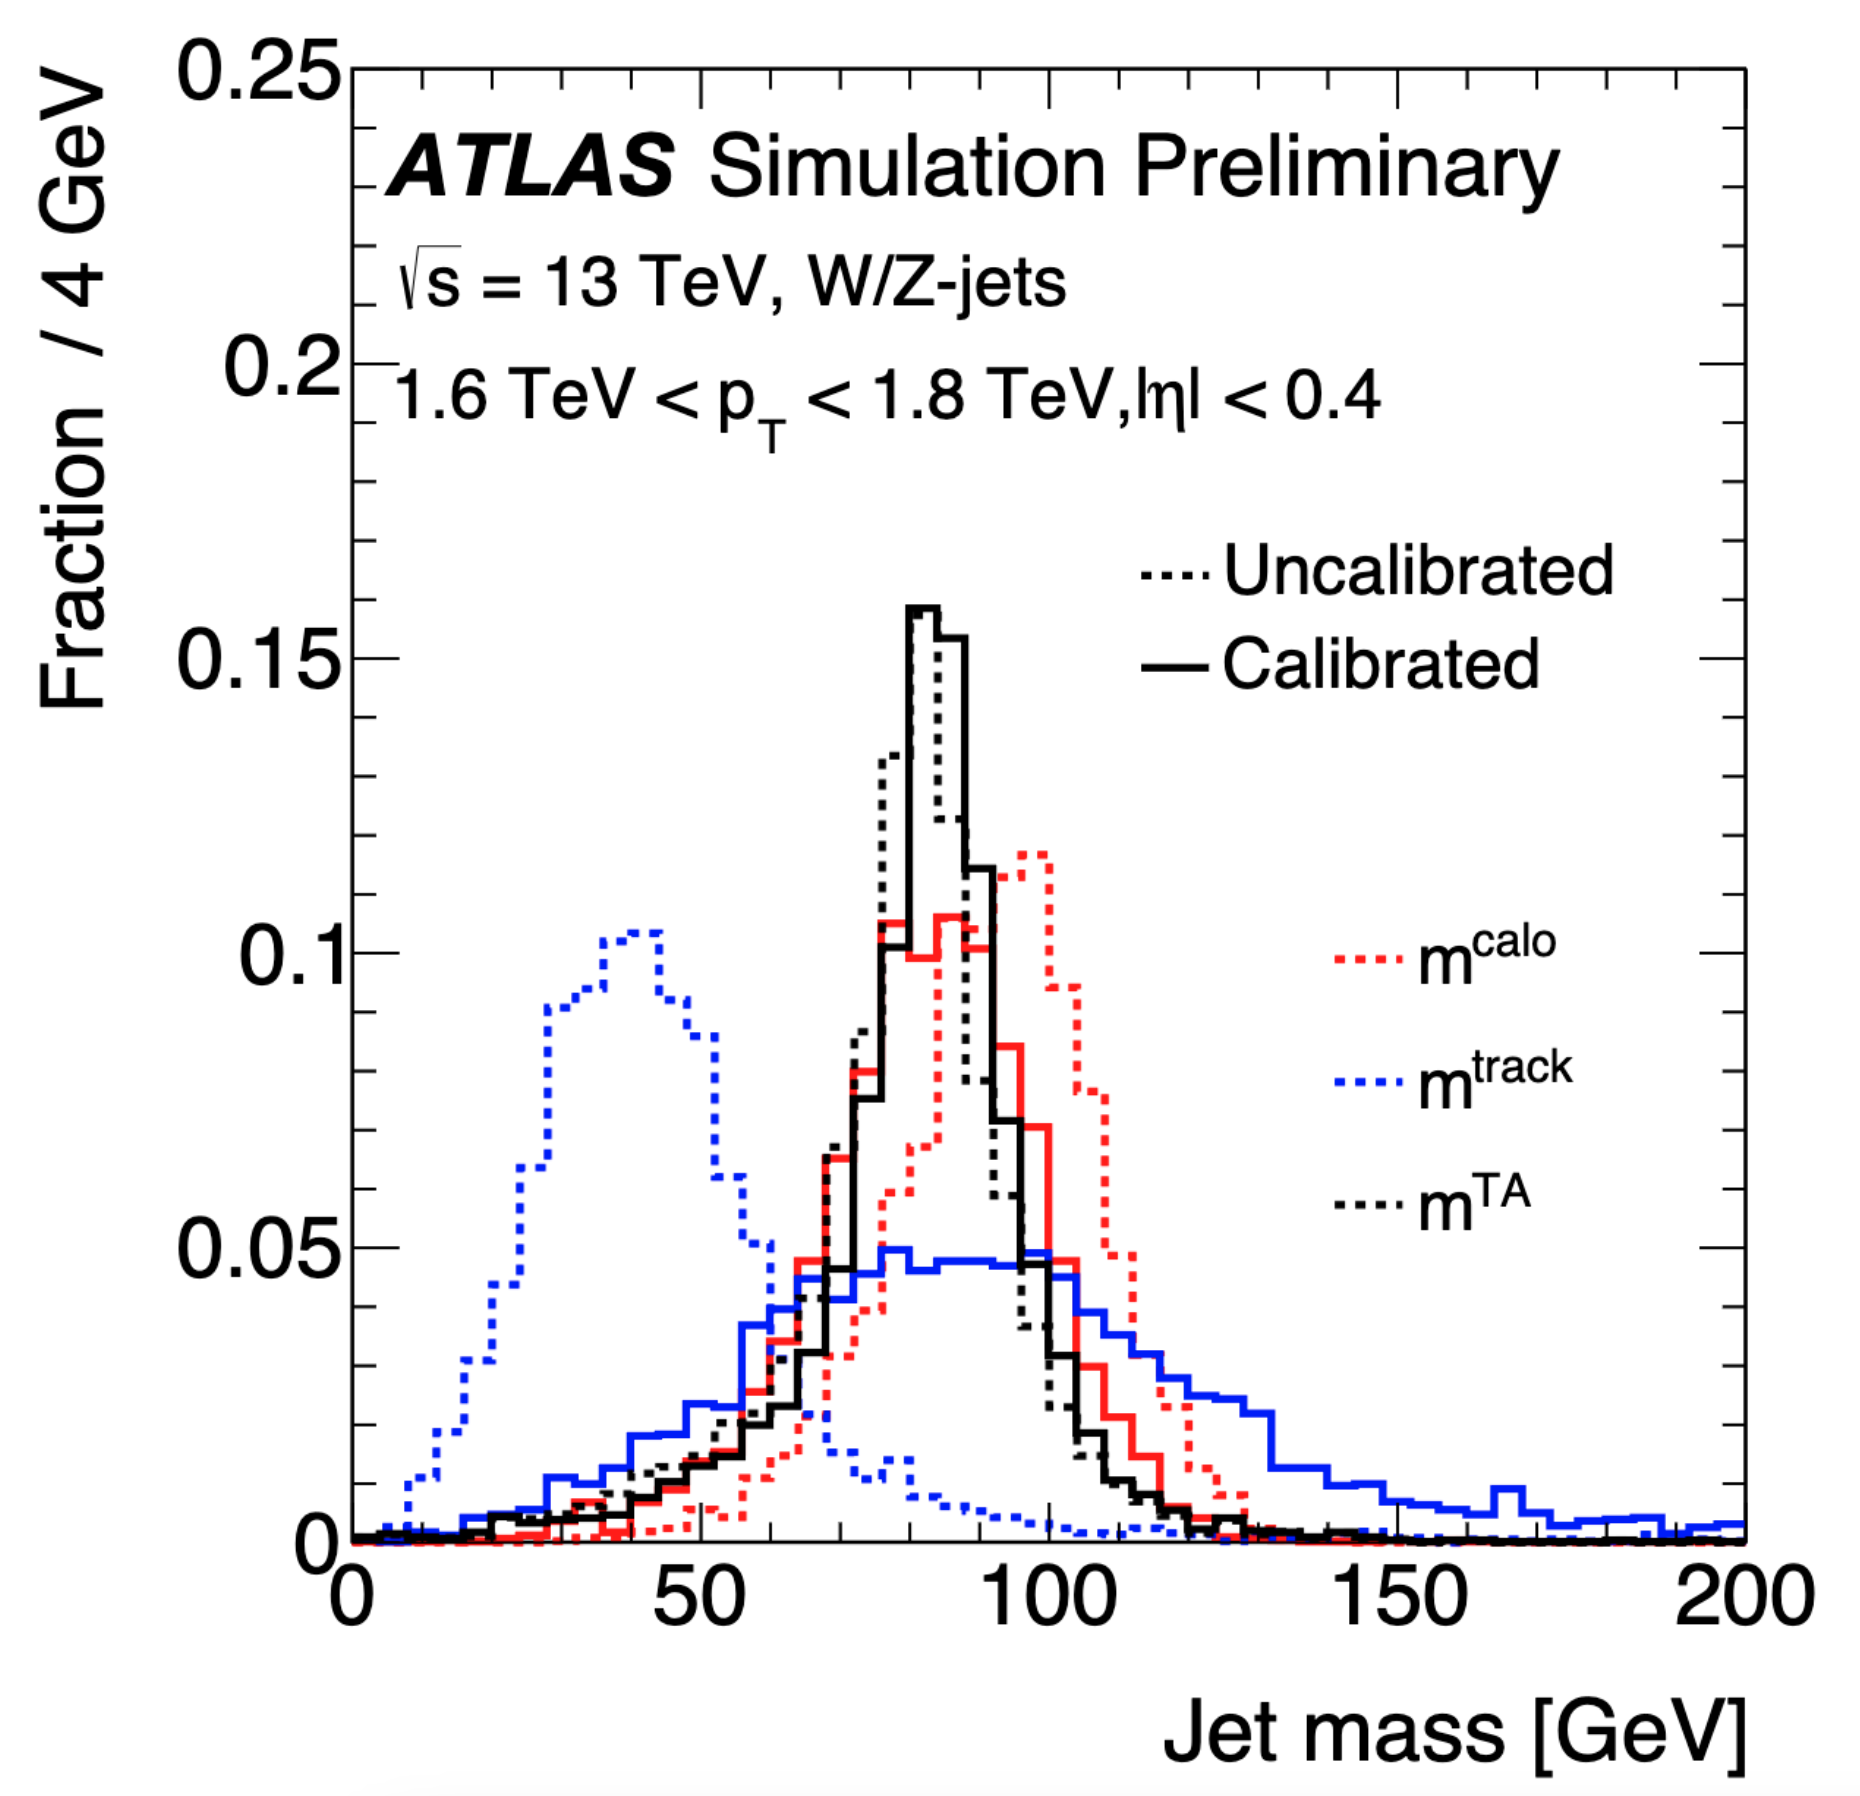
\includegraphics[width=.5\textwidth]{combined_mass_large_R}
  \caption[]{Improvement for track-assisted mass measurement compared to calorimeter and tracking information only. Adopted from \citep{ATLAS-CONF-2016-035} }
  \label{fig:combined_mass_large_R}
\end{figure}
